
\chapter{Proof techniques II --- Induction}
\label{ch:proof2}

{\em Who was the guy who first looked at a cow and said, "I think I'll drink whatever comes out of these things when I squeeze 'em!"? --Bill Watterson}

\section{The principle of mathematical induction}
\label{sec:induct}

The \index{induction}Principle of Mathematical Induction (PMI) may be the least intuitive
proof method available to us.  Indeed, at first, PMI may feel somewhat like
grabbing yourself by the seat of your pants and lifting yourself into
the air.  Despite the indisputable fact that proofs by PMI often feel
like magic, we need to convince you of the validity of this proof
technique.  It is one of the most important tools in your mathematical
kit!

The simplest argument in favor of the validity of PMI is simply that it is
axiomatic.  This may seem somewhat unsatisfying, but the axioms for
the natural number system, known as the \index{Peano axioms}Peano axioms,
include one that justifies PMI.  The Peano axioms will not be treated 
thoroughly in this book, but here they are:

\begin{enumerate}
\item[i)] There is a least element of $\Naturals$ that we denote by $0$.
\item[ii)] Every natural number $a$ has a successor denoted by $s(a)$.
(Intuitively, think of $s(a) = a+1$.)
\item[iii)] There is no natural number whose successor is $0$.  (In other
words, -1 isn't in $\Naturals$.)
\item[iv)] Distinct natural numbers have distinct successors.  
($a \neq b \; \implies \; s(a) \neq s(b)$) 
\item[v)] If a subset of the natural numbers contains $0$ and also has the
property that whenever $a \in S$ it follows that $s(a) \in S$, then the
subset $S$ is actually equal to $\Naturals$.   
\end{enumerate}

The last axiom is the one that justifies PMI.  Basically, if $0$ is in
a subset, and the subset has this property about successors\footnote{Whenever a number is in it, the number's successor must be in it.}, then $1$ must
be in it.  But if $1$ is in it, then $1$'s successor ($2$) must be in it.
And so on \ldots  

The subset ends up having every natural number in it.

\begin{exer}
Verify that the following symbolic formulation has the same content
as the version of the 5th Peano axiom given above.
\[ \forall S \subseteq \Naturals \; ( 0 \in S ) \land (\forall a \in \Naturals, a \in S \, \implies s(a) \in S) \implies  \; S=\Naturals \]

\end{exer}
\bigskip

On August 16th 2003, \index{Lihua, Ma}Ma Lihua of Beijing, China earned her place in the 
record books by single-handedly setting up an arrangement of dominoes 
standing on end (actually, the setup took 7 weeks and was almost ruined by
some cockroaches in the Singapore Expo Hall) and toppling them.  
After the first domino was tipped over it took about six minutes
before 303,621 out of the 303,628 dominoes had fallen. (One has to wonder 
what kept those other 7 dominoes upright \ldots)  

\begin{center}
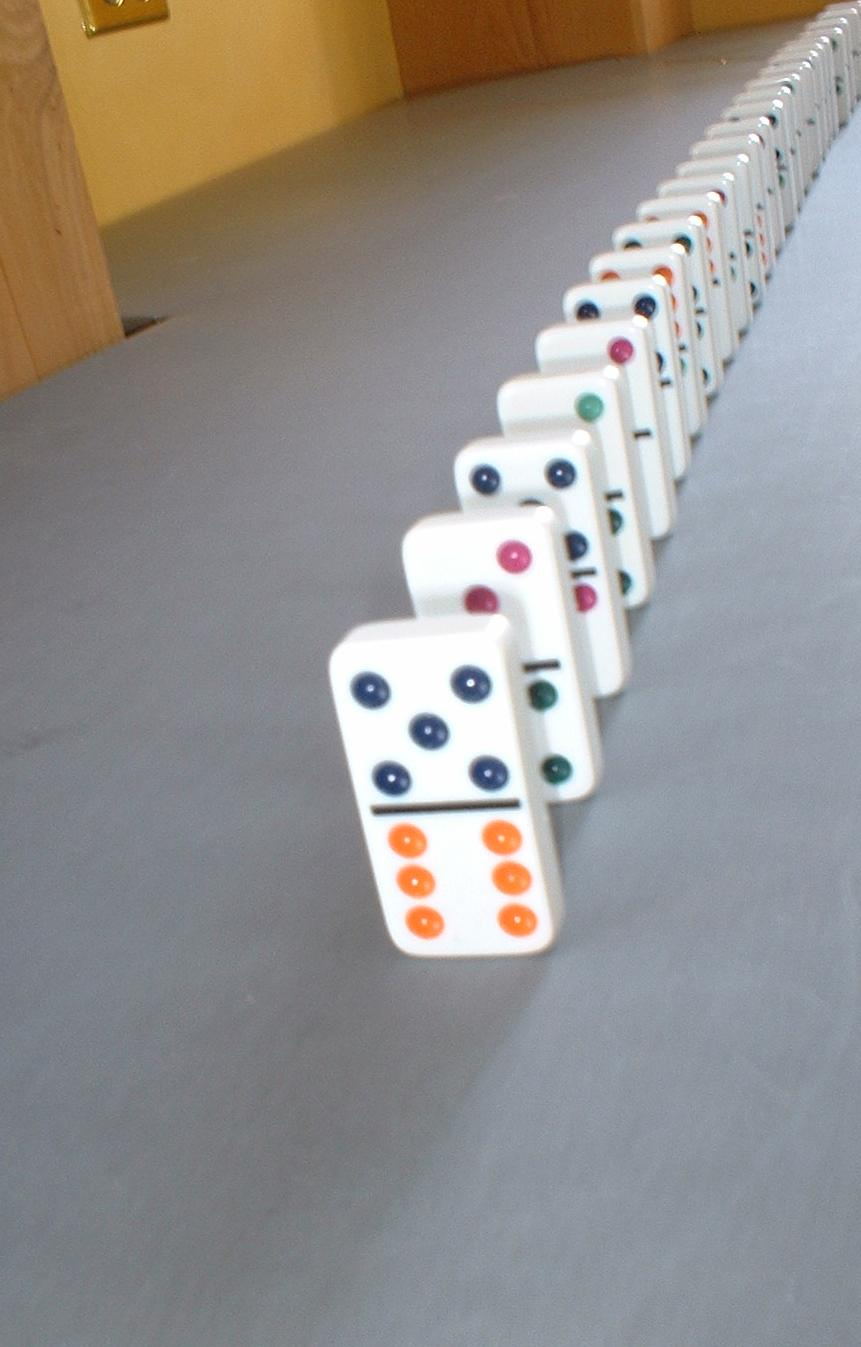
\includegraphics[scale=.2]{photos/domino_row.jpg}
\end{center}

This is the model one should keep in mind when thinking about PMI: domino
toppling.  In setting up a line of dominoes, what do we need to do
in order to ensure that they will all fall when the toppling begins?
Every domino must be placed so that it will hit and topple its successor.
This is exactly analogous to $(a \in S \, \implies s(a) \in S)$.  (Think 
of $S$ having the membership criterion, $x \in S$ = ``$x$ will have fallen
when the toppling is over.'')   The other thing that has to happen
(barring the action of cockroaches) is for someone to knock over the
first domino.  This is analogous to $0 \in S$.

Rather than continuing to talk about subsets of the naturals, it will
be convenient to recast our discussion in terms of infinite families
of logical statements.  If we have a sequence of statements, (one
for each natural number) $P_0$, $P_1$, $P_2$, $P_3$, \ldots  we
can prove them \emph{all} to be true using PMI.  We have to do two
things.   First -- and this is usually the easy part -- we must show 
that $P_0$ is true (i.e. the first domino \emph{will} get knocked over).
Second, we must show, for every possible value of $k$, $P_k \implies P_{k+1}$
(i.e. each domino will knock down its successor).  These two parts 
of an inductive proof are known, respectively, as the \emph{basis}
and the \emph{inductive step}. 

An outline for a proof using PMI:

\begin{center}
\begin{tabular}{|c|} \hline
\rule{16pt}{0pt}\begin{minipage}{.75\textwidth}

\rule{0pt}{16pt}{\bf \large Theorem} $ \displaystyle \forall n \in \Naturals, \; P_n $
\medskip

\rule{0pt}{20pt} {\em Proof:} (By induction)

\noindent {\bf Basis:}

\begin{center}
$\vdots$ \rule{36pt}{0pt} \begin{minipage}[c]{1.7 in} (Here we must show that $P_0$ is true.) \end{minipage}
\end{center}

\noindent {\bf Inductive step:}

\begin{center}
$\vdots$ \rule{36pt}{0pt} \begin{minipage}[c]{1.7 in} (Here we must show that $\forall k,  P_k \implies P_{k+1}$ is true.) \end{minipage}
\end{center}

\rule{0pt}{0pt} \hspace{\fill} Q.E.D. \rule[-10pt]{0pt}{16pt}
\end{minipage} \rule{16pt}{0pt} \\ \hline
\end{tabular}
\end{center}
\medskip

Soon we'll do an actual example of an inductive 
proof, but first we have to say something \emph{REALLY IMPORTANT}
about such proofs.  Pay attention! This is \emph{REALLY IMPORTANT}!
When doing the second part of an inductive proof (the inductive step),
you are proving a UCS, and if you recall how that's done, you start
by assuming the antecedent is true.  But the particular UCS we'll
be dealing with is $\forall k,  P_k \implies P_{k+1}$.  That means
that in the course of proving $\forall n,  P_n$ we have to \emph{assume}
 that $P_k$ is true.  Now this sounds very much like the error known
as ``circular reasoning,'' especially as many authors don't even
use different letters ($n$ versus $k$ in our outline) to distinguish
the two statements.  (And, quite honestly, we only introduced the variable
$k$ to assuage a certain lingering guilt regarding circular reasoning.)
The sentence $\forall n,  P_n$ is what we're trying to prove, but the
sentence we need to prove in order to do that is $\forall k,  P_k \implies P_{k+1}$.
This is subtly different -- in proving that $\forall k,  P_k \implies P_{k+1}$
(which is a UCS!) we assume that $P_k$ is true {\em for some particular value of $k$}.

The sentence $P_k$ is known as the 
\index{inductive hypothesis}\emph{inductive hypothesis}.
Think about it this way:  If we were doing an entirely separate
proof of $\forall n,  P_n \implies P_{n+1}$, it would certainly be fair
to use the inductive hypothesis, and \emph{once that proof was done}, 
it would be okay to quote that result in an inductive proof of 
$\forall n,  P_n$.  Thus we can compartmentalize our way out of the
difficulty!

Okay, so on to an example.  In Section~\ref{sec:basic_set_notions} 
we discovered a formula relating the sizes of a set $A$ and its 
power set ${\mathcal P}(A)$.  If $|A| = n$ then $|{\mathcal P}(A)| = 2^n$.
What we've got here is an infinite family of logical sentences, one for 
each value of $n$ in the natural numbers,

\[ |A| = 0 \implies |{\mathcal P}(A)| = 2^0, \]
\[ |A| = 1 \implies |{\mathcal P}(A)| = 2^1, \]
\[ |A| = 2 \implies |{\mathcal P}(A)| = 2^2, \]
\[ |A| = 3 \implies |{\mathcal P}(A)| = 2^3, \]

\noindent et cetera.

This is exactly the sort of situation in which we use induction.

\begin{thm} For all finite sets $A$, $\displaystyle |A| = n \implies  |{\mathcal P}(A)| = 2^n$.
\end{thm}

\begin{proof}
Let $n = |A|$ and proceed by induction on $n$.

\noindent {\bf Basis:} Suppose $A$ is a finite set and $|A| = 0$, it follows 
that $A = \emptyset$.  The power set of $\emptyset$ is $\{ \emptyset \}$ 
which is a set having 1 element.  Note that $2^0 = 1$.
   
\noindent {\bf Inductive step:}  Suppose that $A$ is a finite set with $|A| = k+1$.  Choose some particular element of $A$, say $a$, and note that
we can divide the subsets of $A$ (i.e. elements of ${\mathcal P}(A)$) into
two categories, those that contain $a$ and those that don't.

Let $S_1 = \{ X \in {\mathcal P}(A) \suchthat a \in X \}$ and let
$S_2 = \{ X \in {\mathcal P}(A) \suchthat a \notin X \}$.  We have 
created two sets that contain all the elements of ${\mathcal P}(A)$,
and which are disjoint from one another.  In symbolic form, 
$S_1 \cup S_2 = {\mathcal P}(A)$ and $S_1 \cap S_2 = \emptyset$.
It follows that $|{\mathcal P}(A)| = |S_1| + |S_2|$.  

Notice that $S_2$ is actually the power set of the $k$-element set
$A \setminus \{ a \}$.  By the inductive hypothesis, $|S_2| = 2^k$.
Also, notice that each set in $S_1$ corresponds uniquely to a set in
$S_2$ if we just remove the element $a$ from it.  This shows that 
$|S_1| = |S_2|$.  Putting this all together we get that 
$|{\mathcal P}(A)| = 2^k + 2^k = 2(2^k) = 2^{k+1}$.

\end{proof}

Here are a few pieces
of advice about proofs by induction:

\begin{itemize}
\item Statements that can be proved inductively don't always start out with 
$P_0$.  Sometimes $P_1$ is the first statement in an infinite family.
Sometimes its $P_5$.  Don't get hung up about something that could be
handled by renumbering things.  
\item In your final write-up you only need to prove the initial case
(whatever it may be) for the basis, but it is a good idea to try 
the first several cases while you are in the ``draft'' stage.  This
can provide insights into how to prove the inductive step, and it may
also help you avoid a classic error in which the inductive approach fails
essentially just because there is a gap between two of the earlier 
dominoes.\footnote{See exercise~\ref{ex:horses}, the classic fallacious proof that all horses are the same color.}
\item It is a good idea to write down somewhere just what it is that
needs to be proved in the inductive step --- just don't make it look like 
you're assuming what needs to be shown.  For instance in the proof above
it might have been nice to start the inductive step with a comment along
the following lines, ``What we need to show is that under the assumption
that any set of size $k$ has a power set of size $2^k$, it follows that
a set of size $k+1$ will have a power set of size $2^{k+1}$.'' 
\end{itemize}
\medskip

We'll close this section with a short discussion about nothing.

\ifthenelse{\boolean{ZeroInNaturals}}{
When we first introduced the natural numbers ($\Naturals$) in Chapter~\ref{ch:intro} we decided to follow the convention that the smallest natural number is 1.
You may have noticed that the Peano axioms mentioned in the beginning of this
section treat $0$ as the smallest natural number.  So, from here on out we
are going to switch things up and side with Dr. Peano.  That is, from now
on we will use the convention

\[\Naturals \, = \, \{ 0, 1, 2, 3, \ldots \} \]

Hmmm\ldots \rule{5pt}{0pt}Maybe that was a short discussion about {\em something} after all.
}{
When we first introduced the natural numbers ($\Naturals$) in Chapter~\ref{ch:intro} we decided to follow the convention that the smallest natural number is 1.
You may have noticed that the Peano axioms mentioned in the beginning of this
section treat $0$ as the smallest natural number.  Many people follow Dr.\ Peano's
convention, but we're going to stick with our original interpretation:

\[\Naturals \, = \, \{ 1, 2, 3, \ldots \} \]

\renewcommand{\Naturals}{{\mathbb Z}^{\mbox{\tiny noneg}} }

Despite our stubbornness, we are forced to admit that many inductive proofs are
made easier by treating the ``first'' case as being in truth the one numbered $0$.   We'll
use the symbol $\Naturals$ to indicate the set ${\mathbb N} \cup \{ 0 \}$.
}

\newpage

  
\noindent{\large \bf Exercises --- \thesection\ }

\begin{enumerate}
\item Consider the sequence of number that are 1 greater than a multiple of 4.
(Such numbers are of the form $4j+1$.)

\[ 1, 5, 9, 13, 17, 21, 25, 29, \ldots \]

The sum of the first several numbers in this sequence can be expressed as
a polynomial.

\[ \sum_{j=0}^n 4j+1 = 2n^2 + 3n + 1 \]

Complete the following table in order to provide evidence that the formula
above is correct.

\begin{center}
\begin{tabular}{c|c|c}
$n$ & $\sum_{j=0}^n 4j+1$ & $2n^2 + 3n + 1$ \\ \hline
 0 & $1$ & $1$ \\
 1 & $1 + 5 = 6$ &  $2 \cdot 1^2 + 3 \cdot 1 + 1 = 6$ \\
 2 & $1 + 5 + 9 = \rule{15pt}{0pt}$ \hint{$15$} &  \hint{$2 \cdot 2^2 + 3 \cdot 2 + 1 = 15$}\\
 3 & \hint{$1 + 5 + 9 + 13 = 28$} &  \hint{$2 \cdot 3^2 + 3 \cdot 3 + 1 = 28$}\\
 4 & & \\
\end{tabular}
\end{center}

\hint{I'm leaving the very last one for you to do.}


\item \label{ex:horses} What is wrong with the following inductive proof of
``all horses are the same color.''?

{\bf Theorem} Let $H$ be a set of $n$ horses, all horses in $H$ 
are the same color.

\begin{proof}
We proceed by induction on $n$.

\noindent {\bf Basis: } Suppose $H$ is a set containing 1 horse.  Clearly
this horse is the same color as itself.

\noindent {\bf Inductive step: } Given a set of $k+1$ horses $H$ we can 
construct two sets of $k$ horses.  Suppose $H = \{ h_1, h_2, h_3, \ldots h_{k+1} \}$.  Define $H_a = \{ h_1, h_2, h_3, \ldots h_{k} \}$ (i.e. $H_a$ contains
just the first $k$ horses) and $H_b = \{ h_2, h_3, h_4, \ldots h_{k+1} \}$ 
(i.e. $H_b$ contains the last $k$ horses).  By the inductive hypothesis
both these sets contain horses that are ``all the same color.''  Also,
all the horses from $h_2$ to $h_k$ are in both sets so both $H_a$ and
$H_b$ contain only horses of this (same) color.  Finally, we conclude that
all the horses in $H$ are the same color.

\end{proof}
\medskip
   
\hint{Look carefully at the stage from $n=2$ to $n=3$.}

\hintspagebreak

\item For each of the following theorems, write the statement that must be
proved for the basis -- then prove it, if you can!

\begin{enumerate}
\item The sum of the first $n$ positive integers is $(n^2+n)/2$.

\hint{The sum of the first $0$ positive integers is $(0^2 + 0)/2$.  Or, if you
prefer to start with something rather than nothing: The sum of the first $1$ positive integers
is $(1^2+1)/2$. }

\item The sum of the first $n$ (positive) odd numbers is $n^2$.

\hint{The sum of the first $0$ positive odd numbers is $0^2$.  Or, the sum of the first $1$ positive odd numbers is $1^2$.}

\item If $n$ coins are flipped, the probability that all of them 
are ``heads'' is $1/2^n$.

\hint{If $1$ coin is flipped, the the probability that it is ``heads'' is $1/2$. Or if we try it 
when $n=0$, ``If no coins are flipped the probability that all t=of them are heads is 1.  Does that
make sense to you?  Is it reasonable that we would say it is 100\% certain that all of the coins
are heads in a set that doesn't contain {\em any} coins? }

\item Every $2^n \times 2^n$ chessboard -- with one square removed -- can 
be tiled perfectly\footnote{Here, ``perfectly tiled'' means that every trominoe
covers 3 squares of the chessboard (nothing hangs over the edge) and that every
square of the chessboard is covered by some trominoe.} by L-shaped trominoes.  
(A trominoe is like a domino but 
made up of $3$ little squares.  There are two kinds, straight 
\begin{picture}(0,0)%
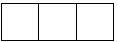
\includegraphics{figures/straight_trominoe.pdf}%
\end{picture}%
\setlength{\unitlength}{3947sp}%
%
\begingroup\makeatletter\ifx\SetFigFont\undefined%
\gdef\SetFigFont#1#2#3#4#5{%
  \reset@font\fontsize{#1}{#2pt}%
  \fontfamily{#3}\fontseries{#4}\fontshape{#5}%
  \selectfont}%
\fi\endgroup%
\begin{picture}(924,324)(1189,-673)
\end{picture}%
 and L-shaped 
\begin{picture}(0,0)%
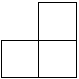
\includegraphics{figures/L-shaped_trominoe.pdf}%
\end{picture}%
\setlength{\unitlength}{3947sp}%
%
\begingroup\makeatletter\ifx\SetFigFont\undefined%
\gdef\SetFigFont#1#2#3#4#5{%
  \reset@font\fontsize{#1}{#2pt}%
  \fontfamily{#3}\fontseries{#4}\fontshape{#5}%
  \selectfont}%
\fi\endgroup%
\begin{picture}(624,624)(1189,-673)
\end{picture}%
. This problem is only concerned with
the L-shaped trominoes.)
\end{enumerate}

\hint{If $n=1$ we have: ``Every $2 \times 2$ chessboard -- with one square removed
can be tiled perfectly by L-shaped trominoes.  This version is trivial to prove.  Try formulating
the $n=0$ case.}
  
\hintspagebreak

\item Suppose that the rules of the game for PMI were changed so that one
did the following:
\begin{itemize}
\item Basis.  Prove that $P(0)$ is true.
\item Inductive step.  Prove that for all $k$, $P_k$ implies $P_{k+2}$
\end{itemize}


\noindent Explain why this would not constitute a valid proof that $P_n$ holds 
for all natural numbers $n$. 
\noindent How could we change the basis in this outline to obtain a valid proof?

\hint{In this modified version, $P(0)$ is not going to imply $P(1)$. and in fact, none of the odd numbered
statements will be proven.  If we change the 
basis so that we prove both $P(0$ and $P(1)$, all the even statements will be implied by
$P(0$ being true and all the odd statements get forced because $P(1)$ is true.}

\item If we wanted to prove statements that were indexed by the integers,

\[ \forall z \in \Integers, \; P_z, \]

\noindent what changes should be made to PMI?

\hint{A quick change would be to replace $\forall k, \; P_k \implies P_{k+1}$ in the inductive
step with $\forall k, \; P_k \iff P_{k+1}$.  While this would do the trick, a slight improvement 
is possible, if we treat the positive and negative cases for $k$ seperately.}
 
\end{enumerate}


%% Emacs customization
%% 
%% Local Variables: ***
%% TeX-master: "GIAM-hw.tex" ***
%% comment-column:0 ***
%% comment-start: "%% "  ***
%% comment-end:"***" ***
%% End: ***



 
\newpage

\section{Formulas for sums and products}
\label{sec:sums_prods}

Gauss, when only a child, found a formula for
summing the first 100 natural numbers (or so the story goes\ldots). 
This formula, and his clever method for justifying it, can be easily 
generalized to the sum of the first $n$ naturals.
While learning calculus, notably during the study of Riemann sums,
one encounters other summation formulas.  For example, in approximating the
integral of the function $f(x)=x^2$ from $0$ to $100$ one needs the sum of 
the first 100 {\em squares}.  For this reason, somewhere in almost
every calculus book one will find the following formulas collected:

\begin{gather*}
\sum_{j=1}^n j = \frac{n(n+1)}{2}\\
\sum_{j=1}^n j^2 = \frac{n(n+1)(2n+1)}{6}\\
\sum_{j=1}^n j^3 = \frac{n^2(n+1)^2}{4}.\\
\end{gather*}

\noindent A really industrious author might also include the sum of the 
fourth powers.  Jacob Bernoulli (a truly industrious individual)
got excited enough to find formulas for the sums of the first
ten powers of the naturals.  Actually, Bernoulli went much further.  His work
on sums of powers lead to the definition of what are now known as Bernoulli
numbers and let him calculate $\sum_{j=1}^{1000}j^{10}$ in 
about seven minutes --
long before the advent of calculators!  In \cite[p. 320]{struik}, Bernoulli is 
quoted:

\begin{quote}
With the help of this table it took me less than half of a quarter of an hour
to find that the tenth powers of the first 1000 numbers being added together 
will yield the sum 

\[ 91,409,924,241,424,243,424,241,924,242,500. \]

\end{quote}

To the beginning calculus student, the beauty of the above relationships may
be somewhat dimmed by the memorization challenge that they represent.  It
is fortunate then, that the right-hand side of the third formula is just 
the square of the right-hand side of the first formula.  And of course,
the right-hand side of the first formula is something that can be deduced 
by a six year old child (provided that he is a super-genius!)  This happy
coincidence leaves us to apply most of our rote memorization energy to
formula number two, because the first and third formulas are related by
the following rather bizarre-looking equation,

\[
\sum_{j=1}^n j^3 = \left( \sum_{j=1}^n j \right)^2. 
\]       

\noindent The sum of the cubes of the first $n$ numbers is the square of their sum.

For completeness we should include the following formula which 
should be thought of as the sum of the zeroth powers of the first $n$
naturals.

\[ \sum_{j=1}^n 1 = n \]

\begin{exer}
Use the above formulas to approximate the integral

\[ \int_{x=0}^{10} x^3 - 2x +3 \mbox{d}x \]
\end{exer}
\bigskip

Our challenge today is not to merely memorize these formulas but
to prove their validity.  We'll use PMI.

Before we start in on a proof, it's important to figure out where 
we're trying to go.  In proving the formula that Gauss discovered
by induction we need to show that the $k+1$--th version of the 
formula holds, assuming that the $k$--th version does.  Before
proceeding on to read the proof do the following

\begin{exer}
Write down the $k+1$--th version of the formula for the sum of
the first $n$ naturals.  (You have to replace every $n$ with 
a $k+1$.)
\end{exer}

\begin{thm}
\[ \forall n \in \Naturals, \; \sum_{j=1}^n j = \frac{n(n+1)}{2} \]
\end{thm}

\begin{proof}
We proceed by induction on $n$.

\noindent {\bf Basis: }  Notice that when $n=0$ the sum on the left-hand side
has no terms in it!  This is known as an \index{empty sum} empty sum, and by 
definition, an empty sum's value is $0$.   Also, when 
$n=0$ the formula on the right-hand side becomes $(0 \cdot 1)/2$ and this is 
$0$ as well.\footnote{If you'd prefer to avoid the ``empty sum'' argument, %
you can choose to use $n=1$ as the basis case.  The theorem should %
be restated so the universe of discourse is \emph{positive} naturals.}

\noindent {\bf Inductive step: }  Consider the sum on the left-hand side of
the $k+1$--th version of our formula.

\[ \sum_{j=1}^{k+1} j \]

We can separate out the last term of this sum.

\[ = (k+1) + \sum_{j=1}^{k} j \]

Next, we can use the inductive hypothesis to replace the sum (the part 
that goes from 1 to $k$) with a formula.

\[ = (k+1) + \frac{k(k+1)}{2} \]

From here on out it's just algebra \ldots

\[ = \frac{2(k+1)}{2} + \frac{k(k+1)}{2} \]

\[ = \frac{2(k+1) + k(k+1)}{2} \]

\[ = \frac{(k+1) \cdot (k+2)}{2}. \]

\end{proof}
\medskip

Notice how the inductive step in this proof works.  We start by writing
down the left-hand side of $P_{k+1}$, we pull out the last term
so we've got the left-hand side of $P_{k}$ (plus something else), then
we apply the inductive hypothesis and do some algebra until we arrive
at the right-hand side of $P_{k+1}$.  Overall, we've just transformed the
left-hand side of the statement we wish to prove into its right-hand side.

There is another way to organize the inductive steps in proofs like these
that works by manipulating entire equalities (rather than just one side
or the other of them).

\begin{quote}

\noindent {\bf Inductive step (alternate): }  By the inductive 
hypothesis, we can write

\[ \sum_{j=1}^{k} j = \frac{k(k+1)}{2}. \]

Adding $(k+1)$ to both side of this yields

\[ \sum_{j=1}^{k+1} j = (k+1) + \frac{k(k+1)}{2}. \]

Next, we can simplify the right-hand side of this to obtain

\[ \sum_{j=1}^{k+1} j = \frac{(k+1)(k+2)}{2}. \]

\rule{0pt}{0pt} \hspace{\fill} Q.E.D.
\end{quote}
\medskip

Oftentimes one can save considerable effort in an inductive 
proof by creatively using the factored form during intermediate steps.
On the other hand, sometimes it is easier to just simplify everything
completely, and also, completely simplify the expression on the 
right-hand side of $P(k+1)$ and then verify that the two things are
equal.  This is basically just another take on the technique of 
``working backwards from the conclusion.''  Just remember that 
in writing-up your proof you need to make it look as if you reasoned
directly from the premises to the conclusion.  We'll illustrate
what we've been discussing in this paragraph while proving
the formula for the sum of the squares of the first $n$ positive integers.

\begin{thm}
\[ \forall n \in \Zplus, \; \sum_{j=1}^n j^2 = \frac{n(n+1)(2n+1)}{6} \]
\end{thm}

\begin{proof}
We proceed by induction on $n$.

\noindent {\bf Basis: } When $n = 1$ the sum has only one term, $1^2 = 1$.
On the other hand, the formula is 
$\displaystyle \frac{1(1+1)(2\cdot 1+1)}{6} = 1$.  Since these are equal, the 
basis is proved.

\noindent {\bf Inductive step: }

\begin{tabular}{|ccc|} \hline
 & &\\
 & \begin{minipage}{4 in} 
Before proceeding with the inductive step, in this box, we will
figure out what the right-hand side of our theorem looks like 
when $n$ is replaced with $k+1$:
\begin{gather*}
 \frac{(k+1)((k+1)+1)(2(k+1)+1)}{6} \\
= \frac{(k+1)(k+2)(2k+3)}{6} \\
= \frac{(k^2+3k+2)(2k+3)}{6} \\
= \frac{2k^3+9k^2+13k+6}{6}.
\end{gather*}
\end{minipage} & \\ 
 & & \\ \hline
\end{tabular}


By the inductive hypothesis,

\[ \sum_{j=1}^k j^2 = \frac{k(k+1)(2k+1)}{6}. \]

Adding $(k+1)^2$ to both sides of this equation gives

\[ (k+1)^2 + \sum_{j=1}^k j^2 = \frac{k(k+1)(2k+1)}{6} + (k+1)^2. \]

Thus,

\[ \sum_{j=1}^{k+1} j^2 = \frac{k(k+1)(2k+1)}{6} + \frac{6(k+1)^2}{6}. \]

Therefore,

\begin{gather*}
\sum_{j=1}^{k+1} j^2 = \frac{(k^2+k)(2k+1)}{6} + \frac{6(k^2+2k+1)}{6} \\
 = \frac{(2k^3+3k^2+k)+(6k^2+12k+6)}{6}\\
 = \frac{2k^3+9k^2+13k+6}{6}\\
 = \frac{(k^2+3k+2)(2k+3)}{6}\\
 = \frac{(k+1)(k+2)(2k+3)}{6} \\
 = \frac{(k+1)((k+1)+1)(2(k+1)+1)}{6}.
\end{gather*}

This proves the inductive step, so the result is true.

\end{proof}

Notice how the last four lines of the proof are the same as those in
the box above containing our scratch work?  (Except in the reverse order.)

We'll end this section by demonstrating one more use of this technique.
This time we'll look at a formula for a product rather than a sum.

\begin{thm} $$\forall n \geq 2 \in \Integers, \prod_{j=2}^n \left( 1 - \frac{1}{j^2} \right) \;  = \; \frac{n+1}{2n}. $$
\end{thm}

Before preceding with the proof let's look at an example (although this 
has nothing to do with proving anything, it's really not a bad idea -- it can
keep you from wasting a lot of time trying to prove something that isn't 
actually true!)  When $n = 4$ the product is

\[  \left(1-\frac{1}{2^2}\right) \cdot \left(1-\frac{1}{3^2}\right) \cdot \left(1-\frac{1}{4^2}\right). 
\]

This simplifies to

\[ \left( 1-\frac{1}{4} \right) \cdot \left( 1-\frac{1}{9} \right) \cdot 
\left( 1-\frac{1}{16} \right) \quad = \quad \left( \frac{3}{4} \right) \cdot \left( \frac{8}{9} \right) \cdot \left( \frac{15}{16} \right) \quad = \quad \frac{360}{576}.
\]

The formula on the right-hand side is 

\[ \frac{4+1}{2 \cdot 4} \quad = \frac{5}{8}. \]

Well!  These two expressions are \emph{clearly} not equal to one another\ldots
What?  You say they are?  Just give me a second with my calculator\ldots

Alright then.  I guess we can't dodge doing the proof\ldots

\begin{proof}
(Using mathematical induction on $n$.)

\noindent {\bf Basis: } When $n = 2$ the product has only one term, $1-1/2^2 = 3/4$.
On the other hand, the formula is 
$\displaystyle \frac{2+1}{2\cdot2} = 3/4$.  Since these are equal, the 
basis is proved.

\noindent {\bf Inductive step: }

Let $k$ be a particular but arbitrarily chosen integer such that

\[ \prod_{j=2}^k \left( 1 - \frac{1}{j^2} \right) \;  = \; \frac{k+1}{2k}. \]

Multiplying\footnote{Really, the only reason I'm doing this silly proof is to 
point out to you that when you're doing the inductive step in a proof of a 
formula for a {\bf product}, you don't add to both sides anymore, you {\bf multiply.} You see that, right?  Well, consider yourself to have been pointed out to or \ldots oh, whatever.}  both sides by the $k+1$-th term of the product 
gives

\[ \left( 1 - \frac{1}{(k+1)^2} \right) \; \cdot \; \prod_{j=2}^k \left( 1 - \frac{1}{j^2} \right) \quad  = \quad \frac{k+1}{2k} \; \cdot \; \left( 1 - \frac{1}{(k+1)^2} \right). \]

Thus 

\[ \prod_{j=2}^{k+1} \left( 1 - \frac{1}{j^2} \right) \quad  = \quad \frac{k+1}{2k} \; \cdot \; \left( 1 - \frac{1}{(k+1)^2} \right) \]

\[ = \frac{k+1}{2k} - \frac{(k+1)}{2k(k+1)^2} \]

\[ = \frac{k+1}{2k} - \frac{(1)}{2k(k+1)} \]

\[ = \frac{(k+1)^2 - 1}{2k(k+1)} \]

\[ = \frac{k^2+2k}{2k(k+1)} \]

\[ = \frac{k (k+2)}{2k(k+1)} \]

\[ = \frac{k+2}{2(k+1)}. \]

\end{proof}

\newpage
  
\noindent{\large \bf Exercises --- \thesection\ }

\begin{enumerate}
\item Write an inductive proof of the formula for the sum 
of the first $n$ cubes.

\hint{
\begin{thm*}
\[ \forall n \in \Naturals, \; \sum_{k=1}^n k^3 \;= \; \left( \frac{n(n+1)}{2} \right)^2 \]
\end{thm*}

\begin{proof} (By mathematical induction)

{\bf Base case:} ($n=1$)
For the base case, note that when $n=1$ we have

\[ \sum_{k=1}^n k^3 \; = \; 1 \]

\noindent and 

\[ \left( \frac{n(n+1)}{2} \right)^2  \; = \; 1.\]

{\bf Inductive step:}

Suppose that $m>1$ is an integer such that 

\[ \sum_{k=1}^m k^3 \; = \; \left( \frac{m(m+1)}{2} \right)^2 \]

\noindent Add $(m+1)^3$ to both sides to obtain

\[ (m+1)^3 + \sum_{k=1}^m k^3 \;= \; \left( \frac{m(m+1)}{2} \right)^2 + (m+1)^3. \]

\noindent Thus

\begin{gather*} 
\sum_{k=1}^{m+1} k^3 \;= \; \left( \frac{m^2(m+1)^2}{4} \right) + \frac{4(m+1)^3}{4} \\
\;= \; \left( \frac{m^2(m+1)^2 + 4 (m+1)^3}{4} \right)\\
\; = \; \left( \frac{(m+1)^2 (m^2 + 4(m+1))}{4} \right)\\
\; = \; \left( \frac{(m+1)^2 (m^2 + 4m +4)}{4} \right)\\
\; = \; \left( \frac{(m+1)^2 (m+2)^2}{4} \right)\\
\; = \; \left( \frac{(m+1)(m+2)}{2} \right)^2
\end{gather*}

 \end{proof}
}

\wbvfill

\workbookpagebreak
  
\item Find a formula for the sum of the first $n$ fourth powers.

\hint{\[ \frac{n\cdot(n+1)\cdot(2n+1)\cdot(3n^2+3n-1)}{30}\] } 

\wbvfill

\workbookpagebreak
 
\item The sum of the first $n$ natural numbers is sometimes called
the $n$-th triangular number \index{triangular numbers}$T_n$.  Triangular numbers are so-named
because one can represent them with triangular shaped arrangements 
of dots. 

\begin{center} \begin{picture}(0,0)%
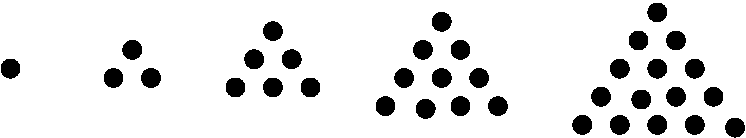
\includegraphics{./triangular_numbers.pdf}%
\end{picture}%
\setlength{\unitlength}{3947sp}%
%
\begingroup\makeatletter\ifx\SetFigFont\undefined%
\gdef\SetFigFont#1#2#3#4#5{%
  \reset@font\fontsize{#1}{#2pt}%
  \fontfamily{#3}\fontseries{#4}\fontshape{#5}%
  \selectfont}%
\fi\endgroup%
\begin{picture}(5963,1088)(1193,-2116)
\end{picture}%
 \end{center}

The first several triangular numbers are 1, 3, 6, 10, 15, et cetera.

Determine a formula for the sum of the first $n$ triangular numbers $\displaystyle \left( \sum_{i=1}^n T_i \right)$ and prove it using PMI.

\hint{The formula is $\frac{n(n+1)(n+2)}{6}$.}

\wbvfill

\workbookpagebreak

\item Consider the alternating sum of squares:
\begin{gather*}
1 \\
1 - 4 = -3 \\
1 - 4 + 9 = 6 \\
1 - 4 + 9 - 16 = -10 \\
\mbox{et cetera}
\end{gather*}
Guess a general formula for $\sum_{i=1}^n (-1)^{i-1} i^2$, and prove it using PMI.

\hint{
\begin{thm*}
\[ \forall n \in \Naturals, \; \sum_{i=1}^n (-1)^{i-1} i^2 \;= \; (-1)^{n-1} \frac{n(n+1)}{2}  \]
\end{thm*}

\begin{proof} (By mathematical induction)

{\bf Base case:} ($n=1$)
For the base case, note that when $n=1$ we have

\[\sum_{i=1}^n (-1)^{i-1} i^2 \;= \; 1 \]

\noindent and also

\[ (-1)^{n-1} \frac{n(n+1)}{2} \;= \; 1. \]

{\bf Inductive step:}

Suppose that $k>1$ is an integer such that 

\[ \sum_{i=1}^k (-1)^{i-1} i^2 \;= \; (-1)^{k-1} \frac{k(k+1)}{2}.  \]

Adding $(-1)^{k} (k+1)^2$ to both sides gives

\begin{gather*} 
\sum_{i=1}^{k+1} (-1)^{i-1} i^2 \;= \; (-1)^{k-1} \frac{k(k+1)}{2} + (-1)^{k} (k+1)^2 \\
\;= \; (-1)^{k-1} \frac{k(k+1)}{2} - (-1)^{k-1} (k+1)^2 \\ 
\;= \; (-1)^{k-1} \left( \frac{k(k+1)}{2} -  \frac{2(k+1)^2}{2} \right) \\ 
\;= \; (-1)^{k} \left( \frac{2(k+1)^2}{2} - \frac{k(k+1)}{2} \right) \\
\;= \; (-1)^{k} \frac{(k+1)(2(k+1)-k)}{2} \\
\;= \; (-1)^{k} \frac{(k+1)(k+2)}{2} \\
\end{gather*}
\end{proof}
}

\wbvfill

\workbookpagebreak

\item Prove the following formula for a product.

\[ \prod_{i=2}^n \left(1 - \frac{1}{i}\right) =  \frac{1}{n} \]

\hint{
Notice that the problem statement didn't specify the domain -- but the smallest value of $n$ that gives
a non-empty product on the left-hand side is $n=2$.  

\newpage

\begin{proof} (By mathematical induction)

{\bf Base case:} ($n=2$)
For the base case, note that when $n=2$ we have

\[ \prod_{i=2}^2 \left(1 - \frac{1}{i}\right) \quad = \quad  \left(1 - \frac{1}{2}\right) \quad = \quad 1/2 \]

\noindent and, when $n=2$, the right-hand side ($1/n$) also evaluates to $1/2$.

{\bf Inductive step:}

Suppose that $k\geq2$ is an integer such that 

\[ \prod_{i=2}^k \left(1 - \frac{1}{i}\right) =  \frac{1}{k}. \]

Then,

\begin{gather*}
\prod_{i=2}^{k+1} \left(1 - \frac{1}{i}\right) \\
= \left(1 - \frac{1}{k+1}\right) \; \cdot \; \prod_{i=2}^{k} \left(1 - \frac{1}{i}\right) \\
= \left(1 - \frac{1}{k+1}\right) \; \cdot \; \frac{1}{k} \\
= \frac{1}{k+1}.
\end{gather*}
\end{proof}

The final line skips over a tiny bit of algebraic detail.  You may feel more comfortable if you fill in those steps.

\newpage
}


\item Prove $\displaystyle \sum_{j=0}^{n}(4j+1) \; = \; 2n^{2}+3n+1$ for all
integers $n \geq 0$.

\hint{
\begin{proof} (By mathematical induction)

{\bf Base case:} ($n=0$)
For the base case, note that when $n=0$ we have

\[ \sum_{j=0}^{n}(4j+1) \; = \; (4\cdot 0 + 1 \; = \; 1 \]

\noindent also, when $n=0$,

\[ 2n^2+3n+1 \; = \; 2\cdot 0^2 +3\cdot 0 + 1 \; = \; 1. \]

{\bf Inductive step:}

Suppose that $k \geq 0$ is an integer such that 

\[  \sum_{j=0}^{k}(4j+1) \; = \; 2k^{2}+3k+1. \]

(We want to show that $\displaystyle \sum_{j=0}^{k+1}(4j+1) \; = \; 2(k+1)^{2}+3(k+1)+1$.)

So consider the sum $\displaystyle \sum_{j=0}^{k+1}(4j+1)$:

\begin{gather*}
\sum_{j=0}^{k+1}(4j+1) \\
= \; 4(k+1)+1 \; + \; \sum_{j=0}^{k}(4j+1) \\
= \;  4(k+1)+1 \; + \; 2k^{2}+3k+1 \\
= \; \rule{0pt}{18pt} \rule{2in}{0pt} \\
= \; \rule{0pt}{18pt} \rule{2in}{0pt} \\
= \; \rule{0pt}{18pt} \rule{2 in}{0pt} \\
\end{gather*}
\end{proof}


Notice that the last line given in the proof is where the inductive hypothesis gets used.  The actual last line of the proof is fairly easy to determine (hint: it is given in the "We want to show" sentence.)  So now you just have to fill in the gaps\ldots

\rule{0pt}{12pt}

}

\wbvfill

\workbookpagebreak

\item Prove $\displaystyle \sum_{i=1}^{n}\frac{1}{(2i-1)(2i+1)} \; = \; \frac{n}{2n+1}$ for all natural numbers $n$.

\hint{
\begin{proof} (By mathematical induction)

{\bf Base case:} ($n=0$)
For the base case, note that when $n=0$ 

\[ \sum_{j=0}^{n} \frac{1}{(2i-1)(2i+1)} \]

contains no terms. Thus its value is 0.

And, $\displaystyle \frac{n}{2n+1}$ also evaluates to 0 when $n=0$.

{\bf Inductive step:}

By the inductive hypothesis we may write

\[ \sum_{i=1}^{k} \frac{1}{(2i-1)(2i+1)} \; = \; \frac{k}{2k+1}. \]

Adding $\displaystyle  \frac{1}{(2(k+1)-1)(2(k+1)+1)}$ to both side of this gives

\[ \sum_{i=1}^{k+1} \frac{1}{(2i-1)(2i+1)} \; = \; \frac{k}{2k+1} \; + \; \frac{1}{(2(k+1)-1)(2(k+1)+1)}. \]

To complete the proof we must verify that 

\[ \frac{k}{2k+1} \; + \; \frac{1}{(2(k+1)-1)(2(k+1)+1)} = \frac{k+1}{2(k+1)+1}. \]

Note that
\begin{gather*}
\rule{0pt}{23pt} \frac{k}{2k+1} \; + \; \frac{1}{(2(k+1)-1)(2(k+1)+1)} \\
\rule{0pt}{23pt} = \frac{k}{2k+1} \; + \; \frac{1}{(2k+1)(2k+3)}\\
\rule{0pt}{23pt} = \frac{k(2k+3)}{(2k+1)(2k+3)} \; + \; \frac{1}{(2k+1)(2k+3)}\\
\rule{0pt}{23pt} = \frac{k(2k+3)+1}{(2k+1)(2k+3)} \\
\rule{0pt}{23pt} = \frac{2k^2+3k+1}{(2k+1)(2k+3)} \\
\rule{0pt}{23pt} = \frac{(2k+1)(k+1)}{(2k+1)(2k+3)} \\
\rule{0pt}{23pt} = \frac{k+1}{2k+3} \; = \; \frac{k+1}{2(k+1)+1}
\end{gather*}

\noindent as desired.


\end{proof}

}
\wbvfill

\workbookpagebreak

\item The \index{Fibonacci numbers} \emph{Fibonacci numbers} are a sequence of integers defined by
the rule that a number in the sequence is the sum of the two that 
precede it.

\[ F_{n+2} = F_n + F_{n+1}  \]

\noindent The first two Fibonacci numbers (actually the zeroth and the first) 
are both 1.  

\noindent Thus, the first several Fibonacci numbers are

\[ F_0 = 1, F_1=1, F_2=2, F_3=3, F_4=5, F_5=8, F_6=13, F_7=21, \; \mbox{et cetera} \]

Use mathematical induction to prove the following formula involving
Fibonacci numbers.

\[ \sum_{i=0}^n (F_i)^2 \, = \, F_n \cdot F_{n+1} \]

\hint{
\begin{proof} (by induction)

{\bf Base case:} ($n=0$)

For the base case, note that when $n=0$ 

\[ \sum_{i=0}^{n} (F_i)^2 \; = \; 1. \]

And, $\displaystyle F_n \cdot F_{n+1} \; = \; F_0 \cdot F_1 \; = \; 1 \cdot 1 \; = \; 1$. 

{\bf Inductive step:}

By the inductive hypothesis we may write

\[ \sum_{i=0}^k (F_i)^2 \; = \; F_k \cdot F_{k+1}. \]

Adding $(F_{k+1})^2$ to both sides gives

\[ \sum_{i=0}^{k+1} (F_i)^2 \; = \; F_k \cdot F_{k+1} + (F_{k+1})^2. \]

Finally, note that (using factoring and the defining property of the Fibonacci numbers)
we can show that

\begin{gather*}
 F_k \cdot F_{k+1} + (F_{k+1})^2 \\
  = \; F_{k+1} \cdot (F_k + F_{k+1}) \\
  = \; F_{k+1} \cdot F_{k+2}
\end{gather*}

So the inductive step has been proved and the result follows by PMI.
\end{proof}
}

\wbvfill

\workbookpagebreak

\end{enumerate}

%% Emacs customization
%% 
%% Local Variables: ***
%% TeX-master: "GIAM-hw.tex" ***
%% comment-column:0 ***
%% comment-start: "%% "  ***
%% comment-end:"***" ***
%% End: ***


 
\newpage

\section[Other proofs using PMI]{Divisibility statements and other proofs using PMI}
\label{sec:other_pmi}

There is a very famous result known as 
\index{Fermat's little theorem}Fermat's Little Theorem.  
This would probably be abbreviated FLT except for two things.
In science fiction FLT means ``faster than light travel'' and 
there is \emph{another} theorem due to Fermat that goes by
the initials FLT: \index{Fermat's last theorem}Fermat's Last Theorem.  
Fermat's last theorem states that equations of the form $a^n+b^n=c^n$,
where $n$ is a positive natural number, 
only have integer solutions that are trivial (like $0^3+1^3=1^3$) when $n$
is greater than 2.  When $n$ is 1, there are lots of integer solutions.
When $n$ is 2, there are still plenty of integer solutions -- these are the
so-called Pythagorean triples, for example 3,4 \& 5 or 5,12 \& 13.  
It is somewhat unfair that this statement is known as Fermat's last \emph{theorem} since he didn't prove it (or at least we can't be sure that he proved it).
Five years after his death, Fermat's son published a translated\footnote{The
translation from Greek into Latin was done by Claude Bachet.} version of
Diophantus's \emph{Arithmetica} containing his father's notations.  One of
those notations -- near the place where Diophantus was discussing the
equation $x^2+y^2=z^2$ and its solution in whole numbers -- was the statement
of what is now known as Fermat's last theorem as well as the following claim:

\begin{quote}
Cuius rei demonstrationem mirabilem sane detexi hanc marginis exiguitas non caperet.
\end{quote}

In English:

\begin{quote}
I have discovered a truly remarkable proof of this that the margin of this page is too small to contain.
\end{quote}

Between 1670 and 1994 a lot of famous mathematicians worked on FLT but
never found the ``demonstrationem mirabilem.''  Finally in 1994, Andrew Wiles
of Princeton announced a proof of FLT, but in Wiles's own words, his is ``a twentieth century proof'' it can't be the proof Fermat had in mind. 

These days most people believe that Fermat was mistaken.  Probably he thought
a proof technique that works for small values of $n$ could be generalized.  
It remains a tantalizing question, can a proof of FLT using only methods
available in the 17th century be accomplished?  

Part of the reason that so many people spent so much effort on FLT
over the centuries is that Fermat had an excellent record as regards
being correct about his theorems and proofs.  The result known as Fermat's
little theorem is an example of a theorem and proof that Fermat got 
right.  It is probably known as his ``little'' theorem because its 
statement is very short, but it is actually a fairly deep result.

\begin{thm}[Fermat's Little Theorem] 
For every prime number $p$, and for all integers $x$, the $p$-th 
power of $x$ and $x$ itself are congruent mod $p$.  Symbolically:

\[ x^p \equiv x \pmod{p} \]
\end{thm}

A slight restatement of Fermat's little theorem is that $p$ is
always a divisor of $x^p-x$ (assuming $p$ is a prime and $x$ is an integer).
Math professors enjoy using their knowledge of Fermat's little theorem
to cook up divisibility results that can be proved using mathematical
induction.   For example, consider the following:

\[ \forall n \in \Naturals,  3 \divides (n^3 + 2n + 6). \]  

This is really just the $p=3$ case of Fermat's little theorem 
with a little camouflage added: $n^3 + 2n + 6 = (n^3-n)+3(n+2)$.
But let's have a look at proving this statement using PMI. 

\begin{thm} 
$\forall n \in \Naturals,  3 \divides (n^3 + 2n + 6)$
\end{thm}

\begin{proof}
(By mathematical induction)

{\bf Basis:} Clearly $3 \divides 6$.

{\bf Inductive step:} 

\noindent (We need to show that $3 \divides (k^3 + 2k + 6) \; \implies \; 3 \divides ((k+1)^3 + 2(k+1) + 6$.)

Consider the quantity $(k+1)^3 + 2(k+1) + 6$.

\begin{gather*}
   (k+1)^3 + 2(k+1) + 6 \\
 = (k^3 + 3k^2 + 3k + 1) + (2k + 2) + 6\\
 = (k^3 + 2k + 6) + 3k^2 + 3k + 3\\
 = (k^3 + 2k + 6) + 3(k^2 + k + 1).
\end{gather*}

By the inductive hypothesis, 3 is a divisor of $k^3 + 2k + 6$ so there
is an integer $m$ such that $k^3 + 2k + 6 = 3m$.
Thus,

\begin{gather*}
(k+1)^3 + 2(k+1) + 6 \\
= 3m + 3(k^2 + k + 1) \\
= 3(m + k^2 + k + 1).
\end{gather*}

This equation shows that 3 is a divisor of $(k+1)^3 + 2(k+1) + 6$, which
is the desired conclusion.
\end{proof}

\begin{exer}
Devise an inductive proof of the statement, $\forall n \in \Naturals, 5 \divides x^5+4x-10$.
\end{exer}

There is one other subtle trick for devising statements to be
proved by PMI that you should know about.  An example should 
suffice to make it clear.  Notice that $7$ is equivalent to $1 \pmod{6}$,
it follows that any power of $7$ is also $1 \pmod{6}$.  So, if we subtract
$1$ from some power of 7 we will have a number that is divisible by $6$.

The proof (by PMI) of a statement like this requires another subtle little
trick.  Somewhere along the way in the proof you'll need the identity $7=6+1$.

\begin{thm}
\[ \forall n \in \Naturals, \; 6 \divides 7^n-1 \]
\end{thm}

\begin{proof} (By PMI)

{\bf Basis:}  Note that $7^0-1$ is $0$ and also that $6 \divides 0$.

{\bf Inductive step:}  

\noindent (We need to show that if $6 \divides 7^k-1$ then $6 \divides 7^{k+1}-1$.)

\noindent Consider the quantity $7^{k+1}-1$.

\begin{gather*}
7^{k+1}-1 = 7 \cdot 7^k -1 \\
 = (6 + 1) \cdot 7^k - 1 \\
 = 6 \cdot 7^k + 1 \cdot 7^k - 1\\
 = 6(7^k) + (7^k - 1)
\end{gather*}

\noindent By the inductive hypothesis, $6 \divides 7^k - 1$ so there is
an integer $m$ such that $7^k - 1 = 6m$.  It follows that

\[ 7^{k+1}-1 = 6(7^k) + 6m. \]

So, clearly, $6$ is a divisor of $7^{k+1}-1$.

\end{proof}

Mathematical induction 
can often be used to prove inequalities.  There are quite a few examples
of families of statements where there is an inequality for every natural
number.  Often such statements seem to be \emph{obviously} true and yet 
devising a proof can be illusive.  If such is the case, try using PMI.
One hint: it is fairly typical that the inductive step in a PMI proof
of an inequality will involve reasoning that isn't particularly sharp. 
Just remember that if you have an inequality and you make the big
side even bigger, the resulting statement is certainly still true! 

Consider the sequences $2^n$ and $n!$.

\begin{center}
\begin{tabular}{c|ccccc}
$n$   & \rule{6pt}{0pt} 0 \rule{6pt}{0pt} & \rule{6pt}{0pt} 1 \rule{6pt}{0pt} &\rule{6pt}{0pt} 2 \rule{6pt}{0pt} & \rule{6pt}{0pt} 3 \rule{6pt}{0pt} & \\ \hline
$2^n$ & 1 & 2 & 4 & 8 & \\ \hline
$n!$  & 1 & 1 & 2 & 6 & \\
\end{tabular}
\end{center}

As the table illustrates, for small values of $n$, $2^n > n!$.  But from $n=4$
onward the inequality is reversed.

\begin{thm} 
\[ \forall n \geq 4 \in \Naturals, 2^n < n! \]
\end{thm}

\begin{proof} (By mathematical induction)

\noindent {\bf Basis:} When $n=4$ we have $2^4 < 4!$, which is certainly 
true ($16 < 24$).

\noindent {\bf Inductive step:} Suppose that $k$ is a natural number 
with $k > 4$, and that $2^k < k!$.  Multiply the left hand side of this
inequality by $2$ and the right hand side by $k+1$\footnote{It might be %
smoother to justify this step by first proving the lemma that %
$\forall a,b,c,d \in {\mathbb R}^+, \; a<b \land c<d \implies ac < bd$. } 
to get

\[ 2\cdot 2^{k} < (k+1) \cdot k!. \]

\noindent So

\[ 2^{k+1} < (k+1)!. \]

\end{proof}

The observant Calculus student will certainly be aware of the fact
that, asymptotically, exponential functions grow faster than polynomial
functions.  That is, if you have a base $b$ which is greater than 1, the 
function $b^x$ is eventually larger than any polynomial $p(x)$.  This
may seem a bit hard to believe if $b=1.001$ and $p(x) = 500x^{10}$.  The
graph of $y=1.001^x$ is practically indistinguishable from the line $y=1$
(at first), whereas the graph of $y=500x^{10}$ has already reached the 
astronomical value of five trillion ($5,000,000,000,000$) when $x$ is just
$10$.  Nevertheless, the exponential will eventually outstrip the polynomial.
We can use the methods of this section to get started on proving the fact 
mentioned above.  Consider the two sequences $n^2$ and $2^n$. 

\begin{center}
\begin{tabular}{c|ccccccc}
$n$   & \rule{6pt}{0pt} 0 \rule{6pt}{0pt} & \rule{6pt}{0pt} 1 \rule{6pt}{0pt} & \rule{6pt}{0pt} 2 \rule{6pt}{0pt} & \rule{6pt}{0pt} 3 \rule{6pt}{0pt} & \rule{6pt}{0pt} 4 \rule{6pt}{0pt} & \rule{6pt}{0pt} 5 \rule{6pt}{0pt} & \rule{6pt}{0pt} 6 \rule{6pt}{0pt} \\ \hline
$n^2$  & 0 & 1 & 4 & 9 & 16 & 25 & 36 \\ \hline
$2^n$ & 1 & 2 & 4 & 8 & 16 & 32 & 64 \\ 
\end{tabular}
\end{center}

If we think of a ``race'' between the sequences $n^2$ and $2^n$, notice
that $2^n$ starts out with the lead.  The two sequences are tied when 
$n=2$.  Briefly, $n^2$ goes into the lead but they are tied again when
$n=4$.  After that it would appear that $2^n$ recaptures the lead for good.
Of course we're making a rather broad presumption -- is it really true
that $n^2$ never catches up with $2^n$ again?  Well, if we're right 
then the following theorem should be provable:

\begin{thm} 
For all natural numbers $n$, if $n \geq 4$ then $n^2 \leq 2^n$.
\end{thm}
 
\begin{quote} \emph{Proof:}

\noindent {\bf Basis:} When $n=4$ we have $4^2 \leq 2^4$, which is 
true since both numbers are 16.

\noindent {\bf Inductive step:} (In the inductive step we assume
that $k^2 \leq 2^k$ and then show that $(k+1)^2 \leq 2^{k+1}$.)

The inductive hypothesis tells us that 

\[ k^2 \leq 2^k. \]

 
If we add $2k+1$ to the left-hand side of this inequality
and $2^k$ to the right-hand side we will produce the desired
inequality.  Thus our proof will follow provided that
we know that $2k+1 \leq 2^k$.  Indeed, it is sufficient to show
that $2k+1 \leq k^2$ since we already know (by the inductive
hypothesis) that $k^2 \leq 2^k$.

So the result remains in doubt unless you can complete the 
exercise that follows\ldots

\rule{0pt}{0pt} \newline \rule{0pt}{15pt} \hfill Q.E.D.??? \end{quote}


\begin{exer} 
Prove the lemma:  For all $n \in \Naturals$, if $n \geq 4$ then
$2n+1 \leq n^2$.
\end{exer}

\newpage
  
\noindent{\large \bf Exercises --- \thesection\ }


Give inductive proofs of the following 
\begin{enumerate}
\item $\forall x \in \Naturals, \; 3 \divides x^3-x$

\wbvfill

%\workbookpagebreak

\item $\forall x \in \Naturals, \; 3 \divides x^3+5x$

\wbvfill

\workbookpagebreak

\item $\forall x \in \Naturals, \; 11 \divides x^{11}+10x$

\wbvfill

%\workbookpagebreak

\item $\forall n \in \Naturals, \; 3 \divides 4^n-1$

\wbvfill

\workbookpagebreak

\item $\forall n \in \Naturals, \; 6 \divides (3n^{2}+3n-12)$

\wbvfill

%\workbookpagebreak

\item $\forall n \in \Naturals, \; 5 \divides (n^{5}-5n^{3}+14n$

\wbvfill

\workbookpagebreak

\item $\forall n \in \Naturals, \; 4 \divides (13^{n}+4n-1)$

\wbvfill

%\workbookpagebreak

\item $\forall n \in \Naturals, \; 7 \divides 8^n+6$

\wbvfill

\workbookpagebreak

\item $\forall n \in \Naturals, \; 6 \divides 2n^3 - 2n - 14$

\wbvfill

%\workbookpagebreak

\item $\forall n \geq 3 \in \Naturals, \; 3n^2+3n+1 < 2n^3$

\wbvfill

\workbookpagebreak

\item $\forall n > 3 \in \Naturals, \; n^3 < 3^n$

\wbvfill

%\workbookpagebreak

\item $\forall n \geq 3 \in \Naturals, \; n^{3}+3>n^{2}+3n+1$

\wbvfill

\workbookpagebreak

\item $\forall x \geq 4 \in \Naturals, \; x^22^x \leq 4^x$

\wbvfill

%\workbookpagebreak

\end{enumerate}


%% Emacs customization
%% 
%% Local Variables: ***
%% TeX-master: "GIAM-hw.tex" ***
%% comment-column:0 ***
%% comment-start: "%% "  ***
%% comment-end:"***" ***
%% End: ***



\newpage
 
\section{The strong form of mathematical induction}
\label{sec:strong_induct}

The strong form of mathematical induction (a.k.a. the principle of
complete induction, PCI; also a.k.a. course-of-values induction) 
is so-called because the hypotheses one
uses are stronger.  Instead of showing that $P_k \implies P_{k+1}$ in
the inductive step, we get to assume that all the statements numbered
smaller than $P_{k+1}$ are true.  To make life slightly easier we'll
renumber things a little.  The statement that needs to be proved is

\[ \forall k (P_0 \land P_1 \land \ldots \land  P_{k-1}) \implies P_k. \]

 An outline of a strong inductive proof is:

\begin{center}
\begin{tabular}{|c|} \hline
\rule{16pt}{0pt}\begin{minipage}{.75\textwidth}

\rule{0pt}{16pt}{\bf \large Theorem} $ \displaystyle \forall n \in \Naturals, \; P_n $
\medskip

\rule{0pt}{20pt} {\em Proof:} (By complete induction)

\noindent {\bf Basis:}

\begin{center}
$\vdots$ \rule{36pt}{0pt} \begin{minipage}[c]{1.7 in} (Technically, a PCI %
proof doesn't require a basis.   We recommend that you show that $P_0$ %
is true anyway.) \end{minipage}
\end{center}

\noindent {\bf Inductive step:}

\begin{center}
$\vdots$ \rule{36pt}{0pt} \begin{minipage}[c]{1.7 in} (Here we must show that $\forall k,  \left( \bigwedge_{i=0}^{k-1} P_i \right) \implies P_{k}$ is true.) \end{minipage}
\end{center}

\rule{0pt}{0pt} \hspace{\fill} Q.E.D. \rule[-10pt]{0pt}{16pt}
\end{minipage} \rule{16pt}{0pt} \\ \hline
\end{tabular}
\end{center}
\medskip

It's fairly common that we won't truly need all of the statements from $P_0$
to $P_{k-1}$ to be true, but just one of them (and we don't know {\em a priori} 
which one).  The following is a classic result; the proof that all numbers
greater than 1 have prime factors.

\begin{thm} For all natural numbers $n$, $n > 1$ implies $n$ has a prime 
factor.
\end{thm}

\begin{proof} (By strong induction)
Consider an arbitrary natural number $n>1$.  If $n$ is prime then $n$ clearly
has a prime factor (itself), so suppose that $n$ is not prime.  By 
definition, a composite
natural number can be factored, so $n=a \cdot b$ for some pair of natural
numbers $a$ and $b$ which are both greater than 1.  Since $a$ and $b$ are  
factors of $n$ both greater than 1, it follows that $a < n$ (it is also 
true that $b < n$ but we don't need that \ldots).  The inductive hypothesis
can now be applied to deduce that $a$ has a prime factor $p$.  Since
$p \divides a$ and $a \divides n$, by transitivity $p \divides n$.  Thus
$n$ has a prime factor.
\end{proof}
  

\newpage

\noindent{\large \bf Exercises --- \thesection\ }


Give inductive proofs of the following 
\begin{enumerate}
\item A ``postage stamp problem'' is a problem that (typically) asks
us to determine what total postage values can be produced using two
sorts of stamps.  Suppose that you have $3$\cents\  stamps and $7$\cents\ 
stamps, show (using strong induction) that any postage value $12$\cents\ 
or higher can be achieved.  That is, 

\[ \forall n \in \Naturals, n \geq 12 \; \implies \;
\exists x,y \in \Naturals , n = 3x + 7y. \]
 
 \wbvfill

\workbookpagebreak

\item Show that any integer postage of $12 \cents$ or more can be made using
only $4\cents$ and $5\cents$ stamps.

\wbvfill

%\workbookpagebreak

\item The polynomial equation $x^2 = x+1$ has two solutions, 
$\alpha = \frac{1+\sqrt{5}}{2}$ and $\beta = \frac{1-\sqrt{5}}{2}$.
Show that the Fibonacci number $F_n$ is less than or equal to $\alpha^{n}$
for all $n \geq 0$.

\wbvfill

\workbookpagebreak

\end{enumerate}


%% Emacs customization
%% 
%% Local Variables: ***
%% TeX-master: "GIAM-hw.tex" ***
%% comment-column:0 ***
%% comment-start: "%% "  ***
%% comment-end:"***" ***
%% End: ***




%% Emacs customization
%% 
%% Local Variables: ***
%% TeX-master: "GIAM.tex" ***
%% comment-column:0 ***
%% comment-start: "%% "  ***
%% comment-end:"***" ***
%% End: ***

